\subsection{Regional changes of velocity and direction}
\label{sec:regional-variations}

Second differences permit a regional comparison that is insensitive to an added
constant velocity. Their physical scale can be expressed without fitting an exponent.
For the two adjacent interval-mean ground velocities,
\begin{equation}
 \overline{\mathbf v}_1=\frac{\mathbf r(t+\tau)-\mathbf r(t)}{\tau},\qquad
 \overline{\mathbf v}_2=\frac{\mathbf r(t+2\tau)-\mathbf r(t+\tau)}{\tau},\qquad
 D_2(\tau)=\frac{\sqrt{V_2(\tau)}}{\tau}
 =\sqrt{\mathbb E|\overline{\mathbf v}_2-\overline{\mathbf v}_1|^2}.
 \label{eq:variation-velocity-change}
\end{equation}
Thus $D_2$, in \si{\metre\per\second}, measures changes of the mean velocity vector
between adjacent intervals. Both changes of direction and changes of its magnitude
contribute. This identity requires neither stationary increments nor self-similarity.
It does not measure wind speed.

The focused measurement uses all \num{\StatVarParaRegionalFlights} paraglider and
\num{\StatVarHangRegionalFlights} hang-glider flights in the three regional take-off
boxes. It reads the verified common-grid coordinates used by the regional PCA,
without repeating cleaning or limiting the number of flights. Eighteen physical
lags span \SIrange{10}{10000}{\second}; the four display lags agree with the updated
PCA at 10, 100, 1000 and \SI{10000}{\second}. Segment boundaries remain mandatory.

Three support conventions answer different questions. The available-origin curves
use every supported origin for each order separately, spaced by $\tau$ within each
segment. The matched-order comparison uses the same origins and flights for orders
one, two and three, and therefore requires $3\tau$ of continuous support. These
stencils overlap even though consecutive origins are separated by $\tau$. A further
common-origin control uses every 10-s origin supporting a continuous 3000-s window,
and retains that exact set for every order and every lag through \SI{1000}{\second}.
The 1000-s limit is a declared support convention; it avoids selecting only flights
with 30,000-s continuous records merely to compare the smaller scales.

Within each flight, eligible origins are pooled before flights receive equal weight.
The report also retains the pooled-origin result used as a weighting sensitivity.
This distinguishes the estimator here from the pooled-origin PCA in
Sec.~\ref{sec:transport-anisotropy}. Uncertainty uses 500 bootstrap draws of complete
site--day groups, jointly across lags and difference orders. Missing group keys
occur in three Alpine paraglider flights and are treated as singleton groups.
Pointwise 95\% intervals require at least 20 contributing groups and 90\% finite
replicates; this display threshold is not a guarantee of coverage. Regional
RMS-change ratios additionally receive approximate simultaneous 95\% bands over
their supported lag grid, obtained from the bootstrap maximum standardised
log-ratio deviation. The interpretation assumes independently resampleable groups;
dependence across sites, dates or repeated pilots can remain.

\begin{figure}[htbp]
 \centering
 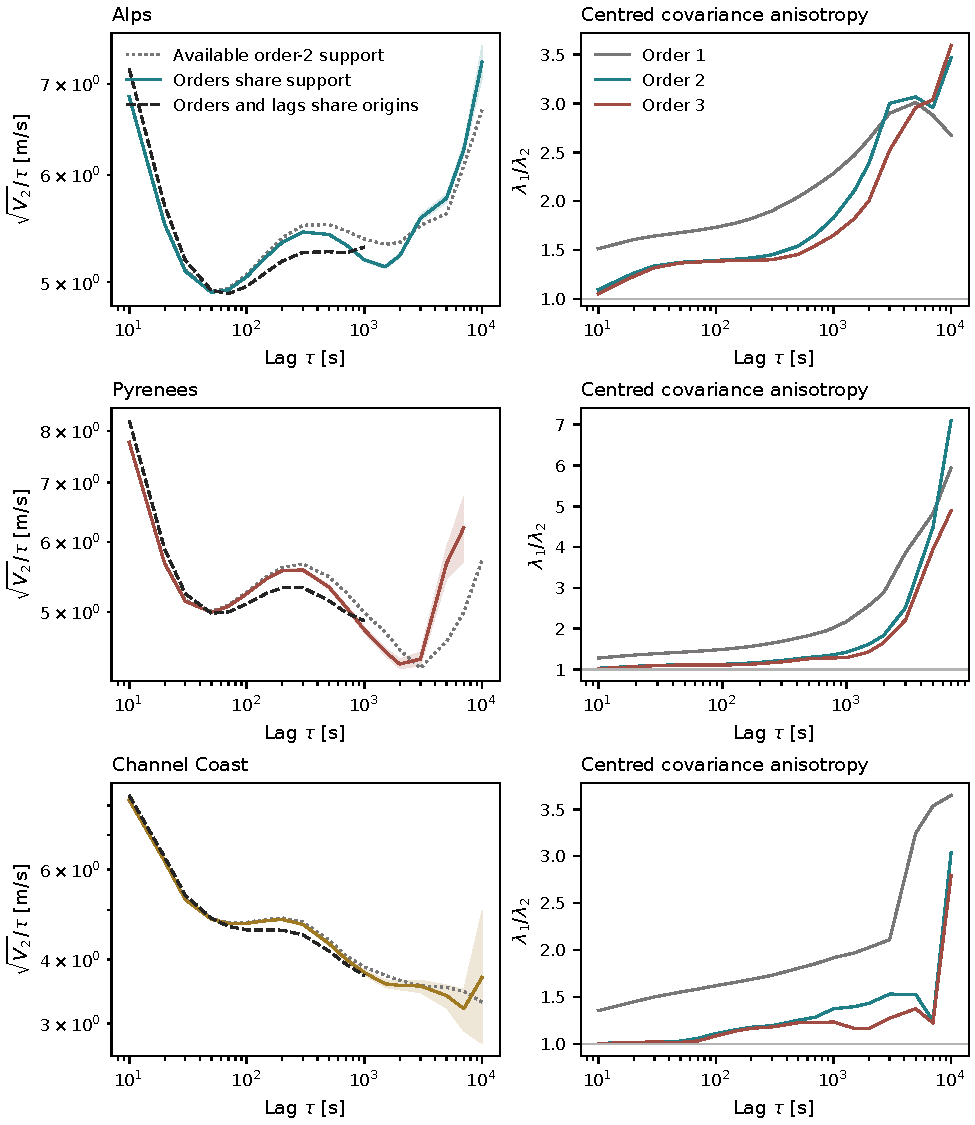
\includegraphics[width=.94\linewidth]{generated/ch3_regional_variations}
 \caption{Regional changes of ground velocity in paragliders. Left: $D_2$ on
 available order-two support, on support shared by orders one to three, and on
 origins common to all orders and lags through 1000~s. Shading is the pointwise
 site--day interval for the matched-order curve. Right: covariance eigenvalue
 ratios on the same matched origins. Curves are omitted where fewer than eight
 flights contribute; all numerical cells remain in the report. Support at the
 long end is shown in Fig.~\ref{fig:variation-support}.}
 \label{fig:regional-variations}
\end{figure}

For directionality, retain the vector $\mathbf d_2=A_2\mathbf r$ before taking its
squared norm. Its mean and centred covariance satisfy
\begin{equation}
 \boldsymbol\mu_2=\mathbb E\mathbf d_2,\qquad
 C_2=\operatorname{Cov}(\mathbf d_2),\qquad
 V_2=\operatorname{tr}C_2+|\boldsymbol\mu_2|^2.
 \label{eq:variation-covariance}
\end{equation}
The covariance includes variation between flight means as well as within flights.
The ratio of its eigenvalues measures directional imbalance of the dispersion;
the scalar $V_2$ alone cannot do so. As before, the leading axis has no signed
direction and becomes poorly determined near equal eigenvalues.

\begin{table}[htbp]
 \centering\small
 \caption{Paraglider diagnostics at \SI{\StatVarReferenceLagS}{\second}, with
 equal flight weights and origins shared by all three difference orders.
 The eigenvalue ratios refer to centred covariances at the indicated order.}
 \label{tab:regional-variations}
 \begin{tabular}{@{}lrrrrr@{}}\toprule
 Region & Flights & $D_2$ [m/s] & Ratio, order 1 & Ratio, order 2 & $V_3/V_2$\\\midrule
 Alps & \num{\StatVarParaAlpsFlights} & \StatVarParaAlpsRmsMatched & \StatVarParaAlpsRatioOne & \StatVarParaAlpsRatioTwo & \StatVarParaAlpsOrderRatio\\
 Pyrenees & \num{\StatVarParaPyreneesFlights} & \StatVarParaPyreneesRmsMatched & \StatVarParaPyreneesRatioOne & \StatVarParaPyreneesRatioTwo & \StatVarParaPyreneesOrderRatio\\
 Channel Coast & \num{\StatVarParaCoastFlights} & \StatVarParaCoastRmsMatched & \StatVarParaCoastRatioOne & \StatVarParaCoastRatioTwo & \StatVarParaCoastOrderRatio\\\bottomrule
 \end{tabular}
\end{table}

At this lag, second differencing reduces the covariance anisotropy relative to
ordinary increments in all three regions, but leaves a directional contrast
(Table~\ref{tab:regional-variations}). The order-two axes are about
\SI{\StatVarParaAlpsAngleTwo}{\degree},
\SI{\StatVarParaPyreneesAngleTwo}{\degree} and
\SI{\StatVarParaCoastAngleTwo}{\degree} counterclockwise from east.
At 10~s the second-difference covariance is much closer to equal principal
variances, especially on the coast; an angle there should not be interpreted as
a resolved environmental orientation.

\begin{figure}[htbp]
 \centering
 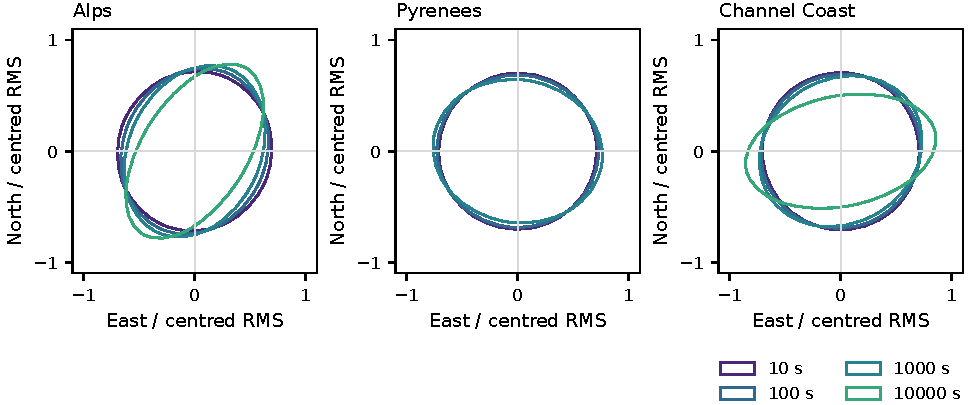
\includegraphics[width=\linewidth]{generated/ch3_variation_axes}
 \caption{Centred second-difference covariance ellipses, normalised by their own
 trace, on matched-order origins. Colours use the same four physical lags as the
 regional PCA. Normalisation removes amplitude and the ellipses omit the mean.
 The Pyrenean 10,000-s ellipse is not shown because only three flights contribute.}
 \label{fig:variation-axes}
\end{figure}

Holding origins fixed through 1000~s gives $D_2$ values of
\SI{\StatVarParaAlpsRmsCommon}{\metre\per\second} in the Alps,
\SI{\StatVarParaPyreneesRmsCommon}{\metre\per\second} in the Pyrenees and
\SI{\StatVarParaCoastRmsCommon}{\metre\per\second} on the coast at 1000~s.
The Alpine-to-coastal ratio is \num{\StatVarParaAlpsVsCoastRatio}, with simultaneous
band \num{\StatVarParaAlpsVsCoastLower}--\num{\StatVarParaAlpsVsCoastUpper}; the
Alpine-to-Pyrenean ratio is \num{\StatVarParaAlpsVsPyreneesRatio}, with band
\num{\StatVarParaAlpsVsPyreneesLower}--\num{\StatVarParaAlpsVsPyreneesUpper}.
The ordering changes with lag: at 10~s the coastal and Pyrenean values exceed the
Alpine value. Similar-looking mountain curves therefore do not establish regional
equality, and a single regional amplitude ratio does not describe the whole interval.

A descriptive standardisation further restricts the common-origin population to
shared strata of declared open/closed task, retained duration (up to 2~h, 2--4~h,
over 4~h), season period (through 2009, 2010--2019, 2020 onward) and equipment
(EN A/B or EN C/D/CCC). Each retained stratum needs at least ten flights per
region; its target mass is proportional to its smallest regional count.
Unknown context labels are excluded from this control. The resulting
\num{\StatVarParaStandardStrata} strata retain
\num{\StatVarParaAlpsStandardFlights}, \num{\StatVarParaPyreneesStandardFlights} and
\num{\StatVarParaCoastStandardFlights} flights. Their standardised 1000-s values
are respectively \SI{\StatVarParaAlpsRmsStandard}{\metre\per\second},
\SI{\StatVarParaPyreneesRmsStandard}{\metre\per\second} and
\SI{\StatVarParaCoastRmsStandard}{\metre\per\second}. The coastal contrast remains
in these point estimates; calibrated intervals for the standardised contrasts are
not supplied. No three-region common equipment/context strata survive for hang gliders.

\begin{figure}[htbp]
 \centering
 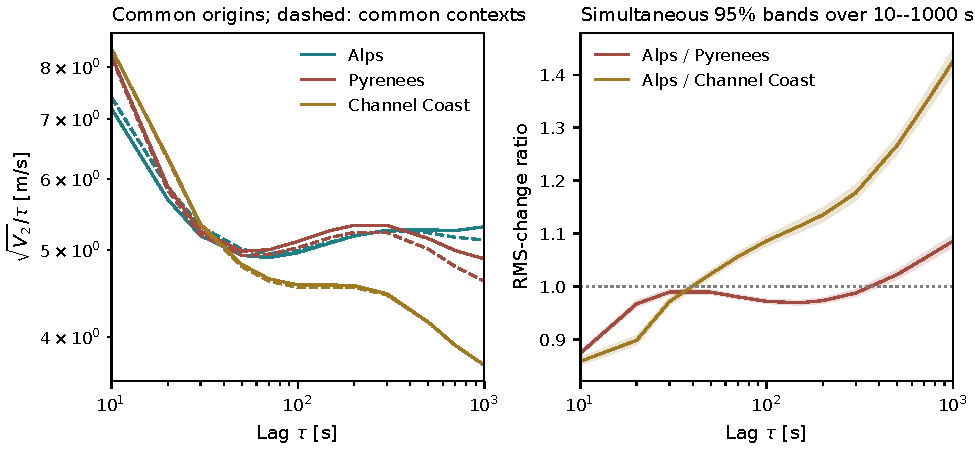
\includegraphics[width=\linewidth]{generated/ch3_variation_controls}
 \caption{Paraglider population controls. Left: common-origin curves, with the
 common-context standardisation dashed. The dashed curves are descriptive point
 estimates. Right: regional ratios of the unstandardised common-origin curves;
 shading is simultaneous over the 18-lag grid's supported subset through 1000~s.
 These controls do not match meteorology, local terrain exposure or pilot identity.}
 \label{fig:variation-controls}
\end{figure}

These findings constrain a wind explanation without identifying wind. If populations
differed only by an added constant velocity and otherwise shared the same residual
dynamics, their second differences would agree. Their measured differences require
more than that particular explanation. Spatial or temporal wind variation, route
geometry, manoeuvres and population selection remain possible contributors. The
coast has smaller changes of interval-mean velocity at 1000~s, rather than a larger
signal that could simply be labelled stronger wind. An environmental attribution
requires independent wind information and terrain alignment, ideally within sites
under contrasting conditions.

\subsection{Third differences and the distribution of changes}
\label{sec:regional-third-differences}

The third difference extends the cancellation by one polynomial degree:
\begin{equation}
 A_3\mathbf r=\mathbf r(t+3\tau)-3\mathbf r(t+2\tau)
              +3\mathbf r(t+\tau)-\mathbf r(t),\qquad
 V_3=\mathbb E|A_3\mathbf r|^2.
 \label{eq:third-difference}
\end{equation}
For $\mathbf r(t)=\mathbf r_0+\mathbf v_0t+\tfrac12\mathbf a t^2$ with constant
vector acceleration, $V_2=|\mathbf a|^2\tau^4$ while $V_3=0$. A smooth curved
trajectory generally retains both signals: locally $A_3\mathbf r$ is proportional
to $\mathbf r^{(3)}\tau^3$. Constant-speed circular motion is therefore not
eliminated by taking order three.

Under the same centred stationary-increment second-moment law used in
Eq.~\eqref{eq:variation-hurst}, algebra gives
\begin{equation}
 V_3=K\bigl(15-6\,2^{2H}+3^{2H}\bigr)\tau^{2H},\qquad
 \frac{V_3}{V_2}=\frac{15-6\,2^{2H}+3^{2H}}{4-2^{2H}},\quad 0<H<1.
 \label{eq:third-difference-hurst}
\end{equation}
The power law must hold through $3\tau$. Thus the order ratio, in addition to the
two slopes, is a consistency condition on that model. It equals three for Brownian
motion plus an arbitrary constant velocity. Agreement between orders would not
constitute independent data or certify removal of every environmental trend.

\begin{figure}[htbp]
 \centering
 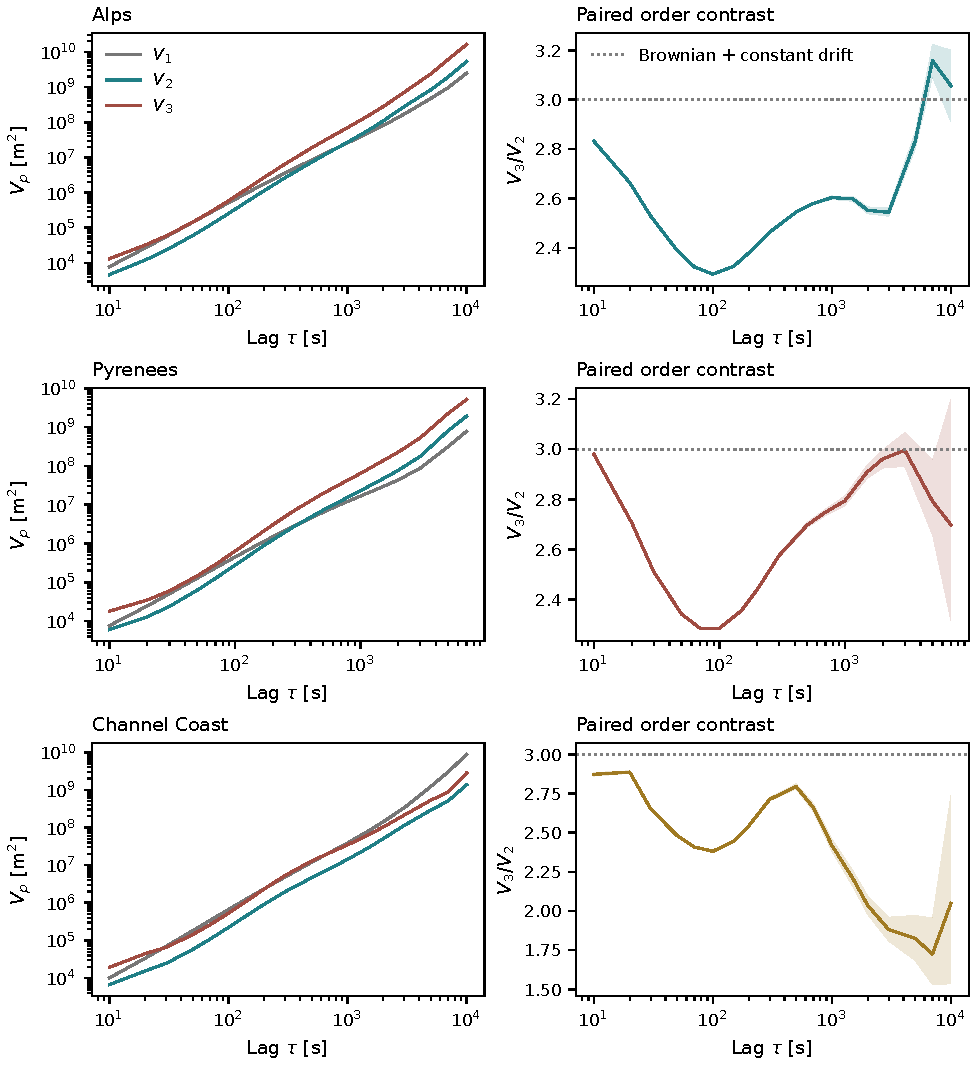
\includegraphics[width=.94\linewidth]{generated/ch3_variation_orders}
 \caption{Paraglider variations and their paired order ratio on identical origins.
 Different prefactors make the amplitudes of $V_2$ and $V_3$ directly unequal even
 under one scaling model. Right: $V_3/V_2$ with pointwise site--day intervals;
 the dotted line is the Brownian-plus-constant-velocity reference, not a fit.
 Fewer than eight contributing flights suppress a displayed curve cell.}
 \label{fig:variation-orders}
\end{figure}

The observed order ratios change with lag (Fig.~\ref{fig:variation-orders}).
At 100~s they are about 2.29 in both mountain regions and 2.38 on the coast;
at 1000~s they are \num{\StatVarParaAlpsOrderRatio},
\num{\StatVarParaPyreneesOrderRatio} and \num{\StatVarParaCoastOrderRatio}.
These curves supply a sensitivity and model-consistency diagnostic, without
establishing a scale-independent Hurst parameter. Order three also increases the
effect of independent position errors: variance $\sigma^2$ per coordinate adds
$6\sigma^2$ to the order-two scalar-component moment and $20\sigma^2$ to order
three. Correlated errors and smoothing alter those expressions. The 10-s end
therefore remains sensitive to acquisition and preprocessing resolution; a
calibrated sensor-noise subtraction is not performed here.

The distribution of $|A_2\mathbf r|/\tau$ supplies information lost by its second
moment. We retain equal-flight histogram probabilities and the squared-change
contribution of every bin, including zeros and both tails. Reported quantiles are
bin bounds, not interpolated exact sample quantiles. At 1000~s, the largest tenth
of changes accounts for approximately
\num{\StatVarParaAlpsTailShareLow}--\num{\StatVarParaAlpsTailShareHigh}\% of the
squared-change signal in the Alps,
\num{\StatVarParaPyreneesTailShareLow}--\num{\StatVarParaPyreneesTailShareHigh}\%
in the Pyrenees and
\num{\StatVarParaCoastTailShareLow}--\num{\StatVarParaCoastTailShareHigh}\% on the
coast. Each range reflects the unresolved boundary bin, not sampling uncertainty.
This measures concentration of the observable; it does not identify a flight
phase, turbulence or a tail-generating mechanism.

\begin{figure}[htbp]
 \centering
 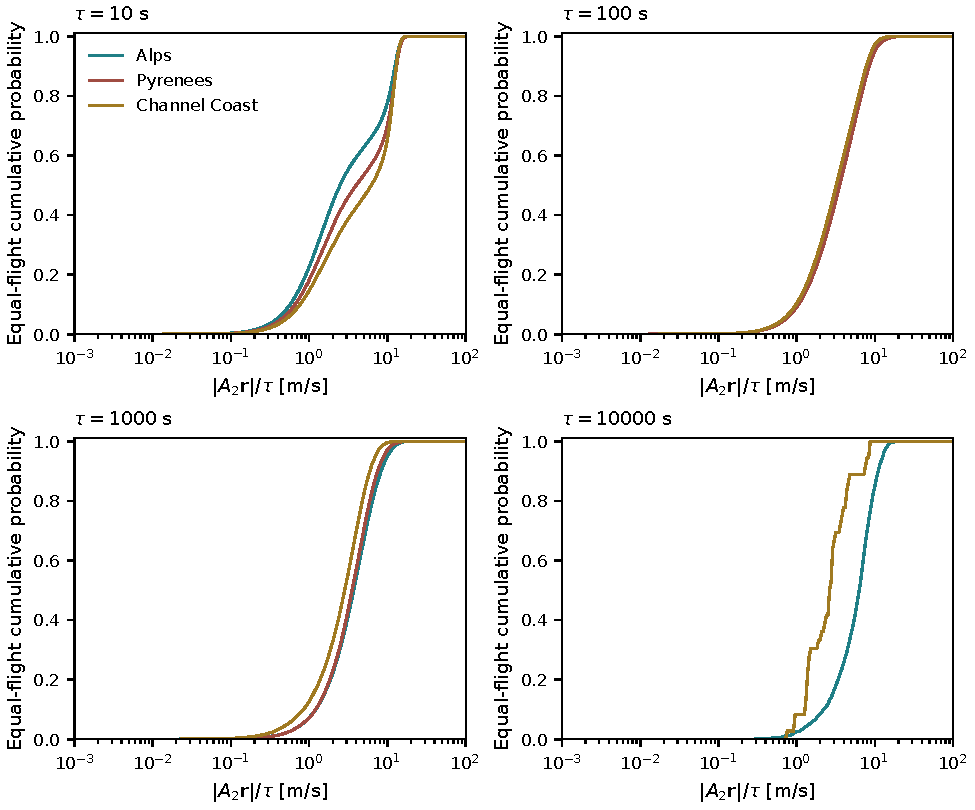
\includegraphics[width=\linewidth]{generated/ch3_variation_distributions}
 \caption{Equal-flight distributions of changes of interval-mean velocity at the
 four PCA display lags, using matched-order support. Curves are accumulated from
 fixed logarithmic bins; the complete report retains zero and overflow mass.
 No distribution is drawn for fewer than eight flights. The changing long-lag
 population must accompany comparisons between panels.}
 \label{fig:variation-distributions}
\end{figure}

\begin{figure}[htbp]
 \centering
 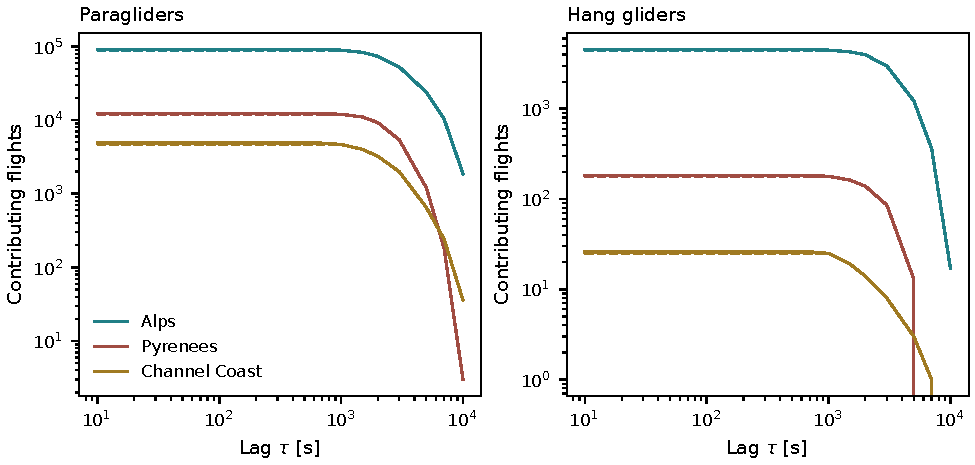
\includegraphics[width=\linewidth]{generated/ch3_variation_support}
 \caption{Contributing flights for matched orders (solid) and common origins
 through 1000~s (dashed). A matched observation requires $3\tau$ of continuous
 support. At 10,000~s the paraglider counts are
 \num{\StatVarParaAlpsMaxFlights}, \num{\StatVarParaPyreneesMaxFlights} and
 \num{\StatVarParaCoastMaxFlights}; hang-glider counts are
 \num{\StatVarHangAlpsMaxFlights}, \num{\StatVarHangPyreneesMaxFlights} and
 \num{\StatVarHangCoastMaxFlights}. All regional eligible flights enter where supported.}
 \label{fig:variation-support}
\end{figure}
